\documentclass{beamer}
\mode<beamer>{%
\usetheme[hideothersubsections,
right,width=22mm]{Goettingen}
}
\usepackage[spanish]{babel} %Definir idioma español
\usepackage[utf8]{inputenc} %Codificacion utf-8
\spanishdecimal{.}
\title{Proyecto de aprendizaje por refuerzo}
\author{Emmanuel Peto Gutiérrez}
\institute{IIMAS \\ UNAM}
\begin{document}

\begin{frame}<handout:0>
\titlepage
\end{frame}

\section{Introducción}

% 1
\begin{frame}
\frametitle{El sistema}

Sistema de tanque de agua con una bomba de entrada y un agujero de salida.

\begin{center}
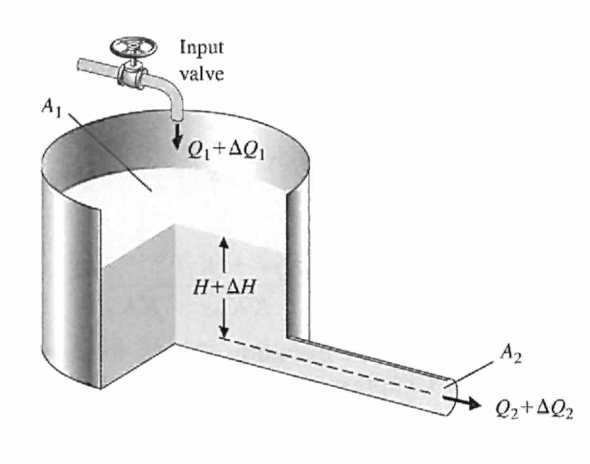
\includegraphics[scale=0.3]{tanque}
\end{center}

\end{frame}

% 2
\begin{frame}
\frametitle{El modelo matemático}

La ecuación diferencial: $$\frac{dH}{dt} = - (\frac{A_2}{A_1}\sqrt{2g})\sqrt{H} + \frac{1}{\rho A_1} Q_1$$

La función de transferencia continua: $$\frac{0.0013}{s+0.0221}$$

La función de transferencia discreta (ts=0.2s): $$\frac{2.5409 \times 10^{-4}}{z-0.9956}$$

La altura en un instante: $$ h^{(i)} = 0.9956 h^{(i-1)} + 2.5409 \times 10^{-4}u $$

\end{frame}

\section{Implementación}

% 3
\begin{frame}
\frametitle{El MDP}

\begin{itemize}
\item \textbf{Estados}: $s \in [0, 2]$ (continuo)
\item \textbf{Acciones}: $a \in [0, 50]$ (continuo)
\item \textbf{Probabilidades}: $p(s', r | s, a) = 1$, donde $s' = 0.9956s + 2.5409 \times 10^{-4}a$.
\item \textbf{Recompensa}: La recompensa es -1 por llegar a un estado no terminal y 200 por llegar a un estado terminal. Un estado terminal se alcanza cuando la altura actual del tanque se acerca a la altura objetivo con un margen de 0.01m.
\item \textbf{Descuento}: $\gamma = 0.99$
\end{itemize}

\end{frame}

% 4
\begin{frame}
\frametitle{El algoritmo}

Se utilizó el algoritmo DQN para entrenar al agente, usando $\epsilon$-greedy para la selección de la acción. Al final se obtiene una red neuronal entrenada, la cual se utiliza para hacer control sobre el sistema y llegar a la altura objetivo.

Los hiperparámetros usados en el algoritmo son
\begin{itemize}
\item $\alpha$: $1 \times 10^{-4}$
\item $\epsilon$: valor decreciente de 1 a 0.01
\item Tamaño de batch: 32
\item Episodios: 1000
\item Pasos (máximos) por episodio: 1000
\end{itemize}

\end{frame}

\section{Resultados}

% 5
\begin{frame}
\frametitle{Recompensa promedio}

En la siguiente gráfica se muestra la recompensa promedio de cada episodio de la fase de entrenamiento.

\begin{center}
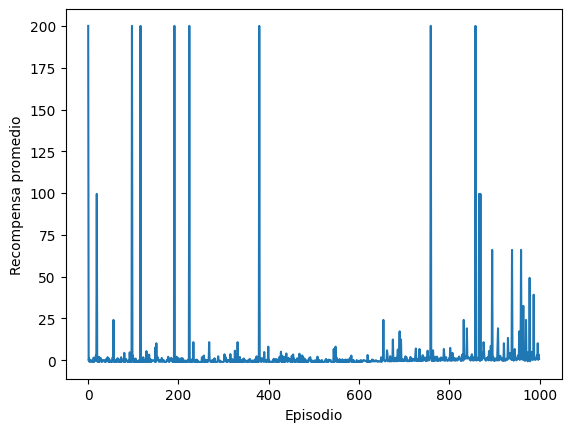
\includegraphics[scale=0.5]{mean_reward.png}
\end{center}

\end{frame}

% 6
\begin{frame}
\frametitle{Control - parte 1}

Fase de control cuando la altura inicial es 0.

\begin{center}
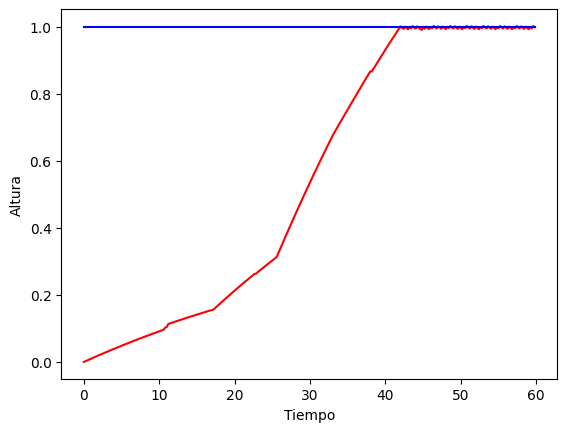
\includegraphics[scale=0.31]{altura_tiempo_p1.png}

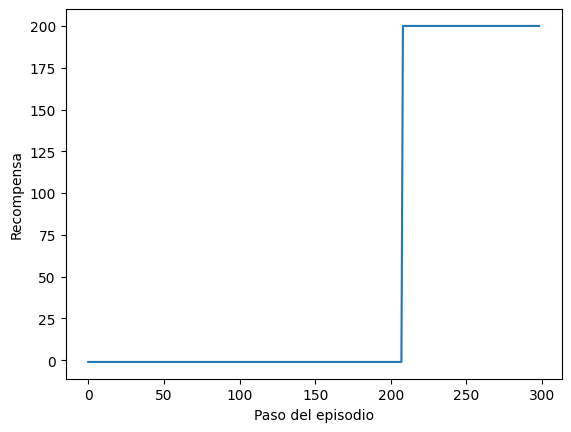
\includegraphics[scale=0.31]{recompensa_pasos_p1.png}
\end{center}

\end{frame}

% 7
\begin{frame}
\frametitle{Control - parte 2}

Fase de control cuando la altura inicial es 1.7.

\begin{center}
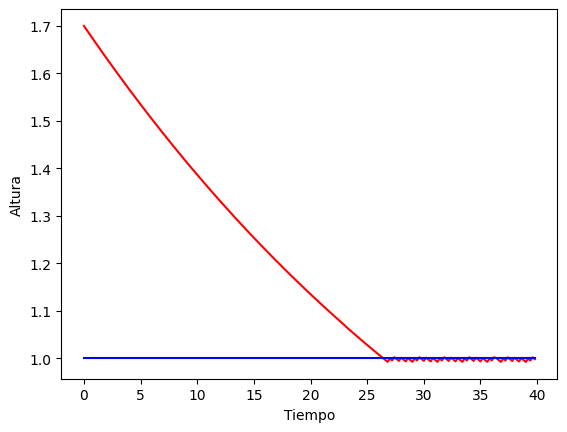
\includegraphics[scale=0.31]{altura_tiempo_p2.png}

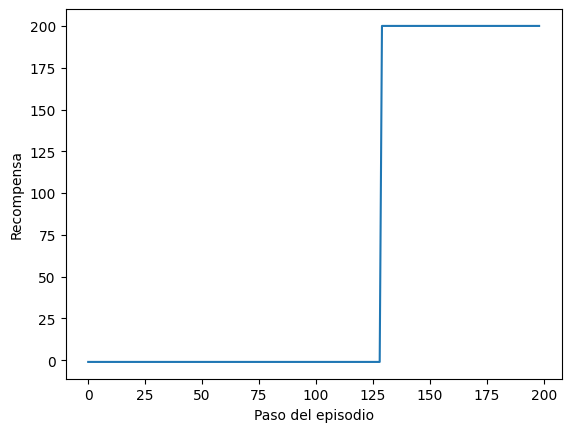
\includegraphics[scale=0.31]{recompensa_pasos_p2.png}
\end{center}

\end{frame}

\end{document}

